\documentclass[a4paper,12pt]{llncs}
\usepackage[top=75pt, bottom=75pt, left=85pt, right=85pt]{geometry}

\usepackage{amssymb}
\setcounter{tocdepth}{3}
\usepackage{graphicx}
\usepackage{soul,color}
\usepackage{url}
\usepackage{algorithm}
\usepackage{enumitem}
\newcommand{\keywords}[1]{\par\addvspace\baselineskip
\noindent\keywordname\enspace\ignorespaces#1}
\newcommand{\ie}{i.e.} 
\newcommand{\eg}{e.g.} 
\newcommand{\et}{et al. }

\begin{document}
\title{Weekly Report -- 48}
\author{Xiufeng Liu}
\institute{University of Waterloo, CA\\
\email{xiufeng.liu@uwaterloo.ca}
}
\maketitle


\section{This Week}
In this week I continue to study the \texttt{ESSEX} data set, and complete the study report. Also, in the group meeting on Wednesday and Thursday, we outlined the route of our research. Before we make a centre data warehouse system for data analysis, we will first continue current work that is to do the benchmark study of energy data on different systems, including Matlab, PostgreSQL+Matlib,  KDB+ and other column stores. 

\section{Next Week}
I will start to investigate the technologies that could integrate the analysis results available, then consider to build a prototype of an web-based analysis platform.  The analytics results from different sources could be easily ``added into" the platform and visualized. This is an on-going project that will be completed progressively to the next year. For the benchmark study, we have to outline the work and take steps in soon.



\section{ESSEX Data}
Fig.~\ref{fig:essex_annotated} shows the database schema of the annotated ESSEX data (The tables colored by blue are the original tables, while the ones colored by purple are the annotated tables). To ease understanding, I have classified the tables into different categories.
\begin{figure}[htp]
\centering
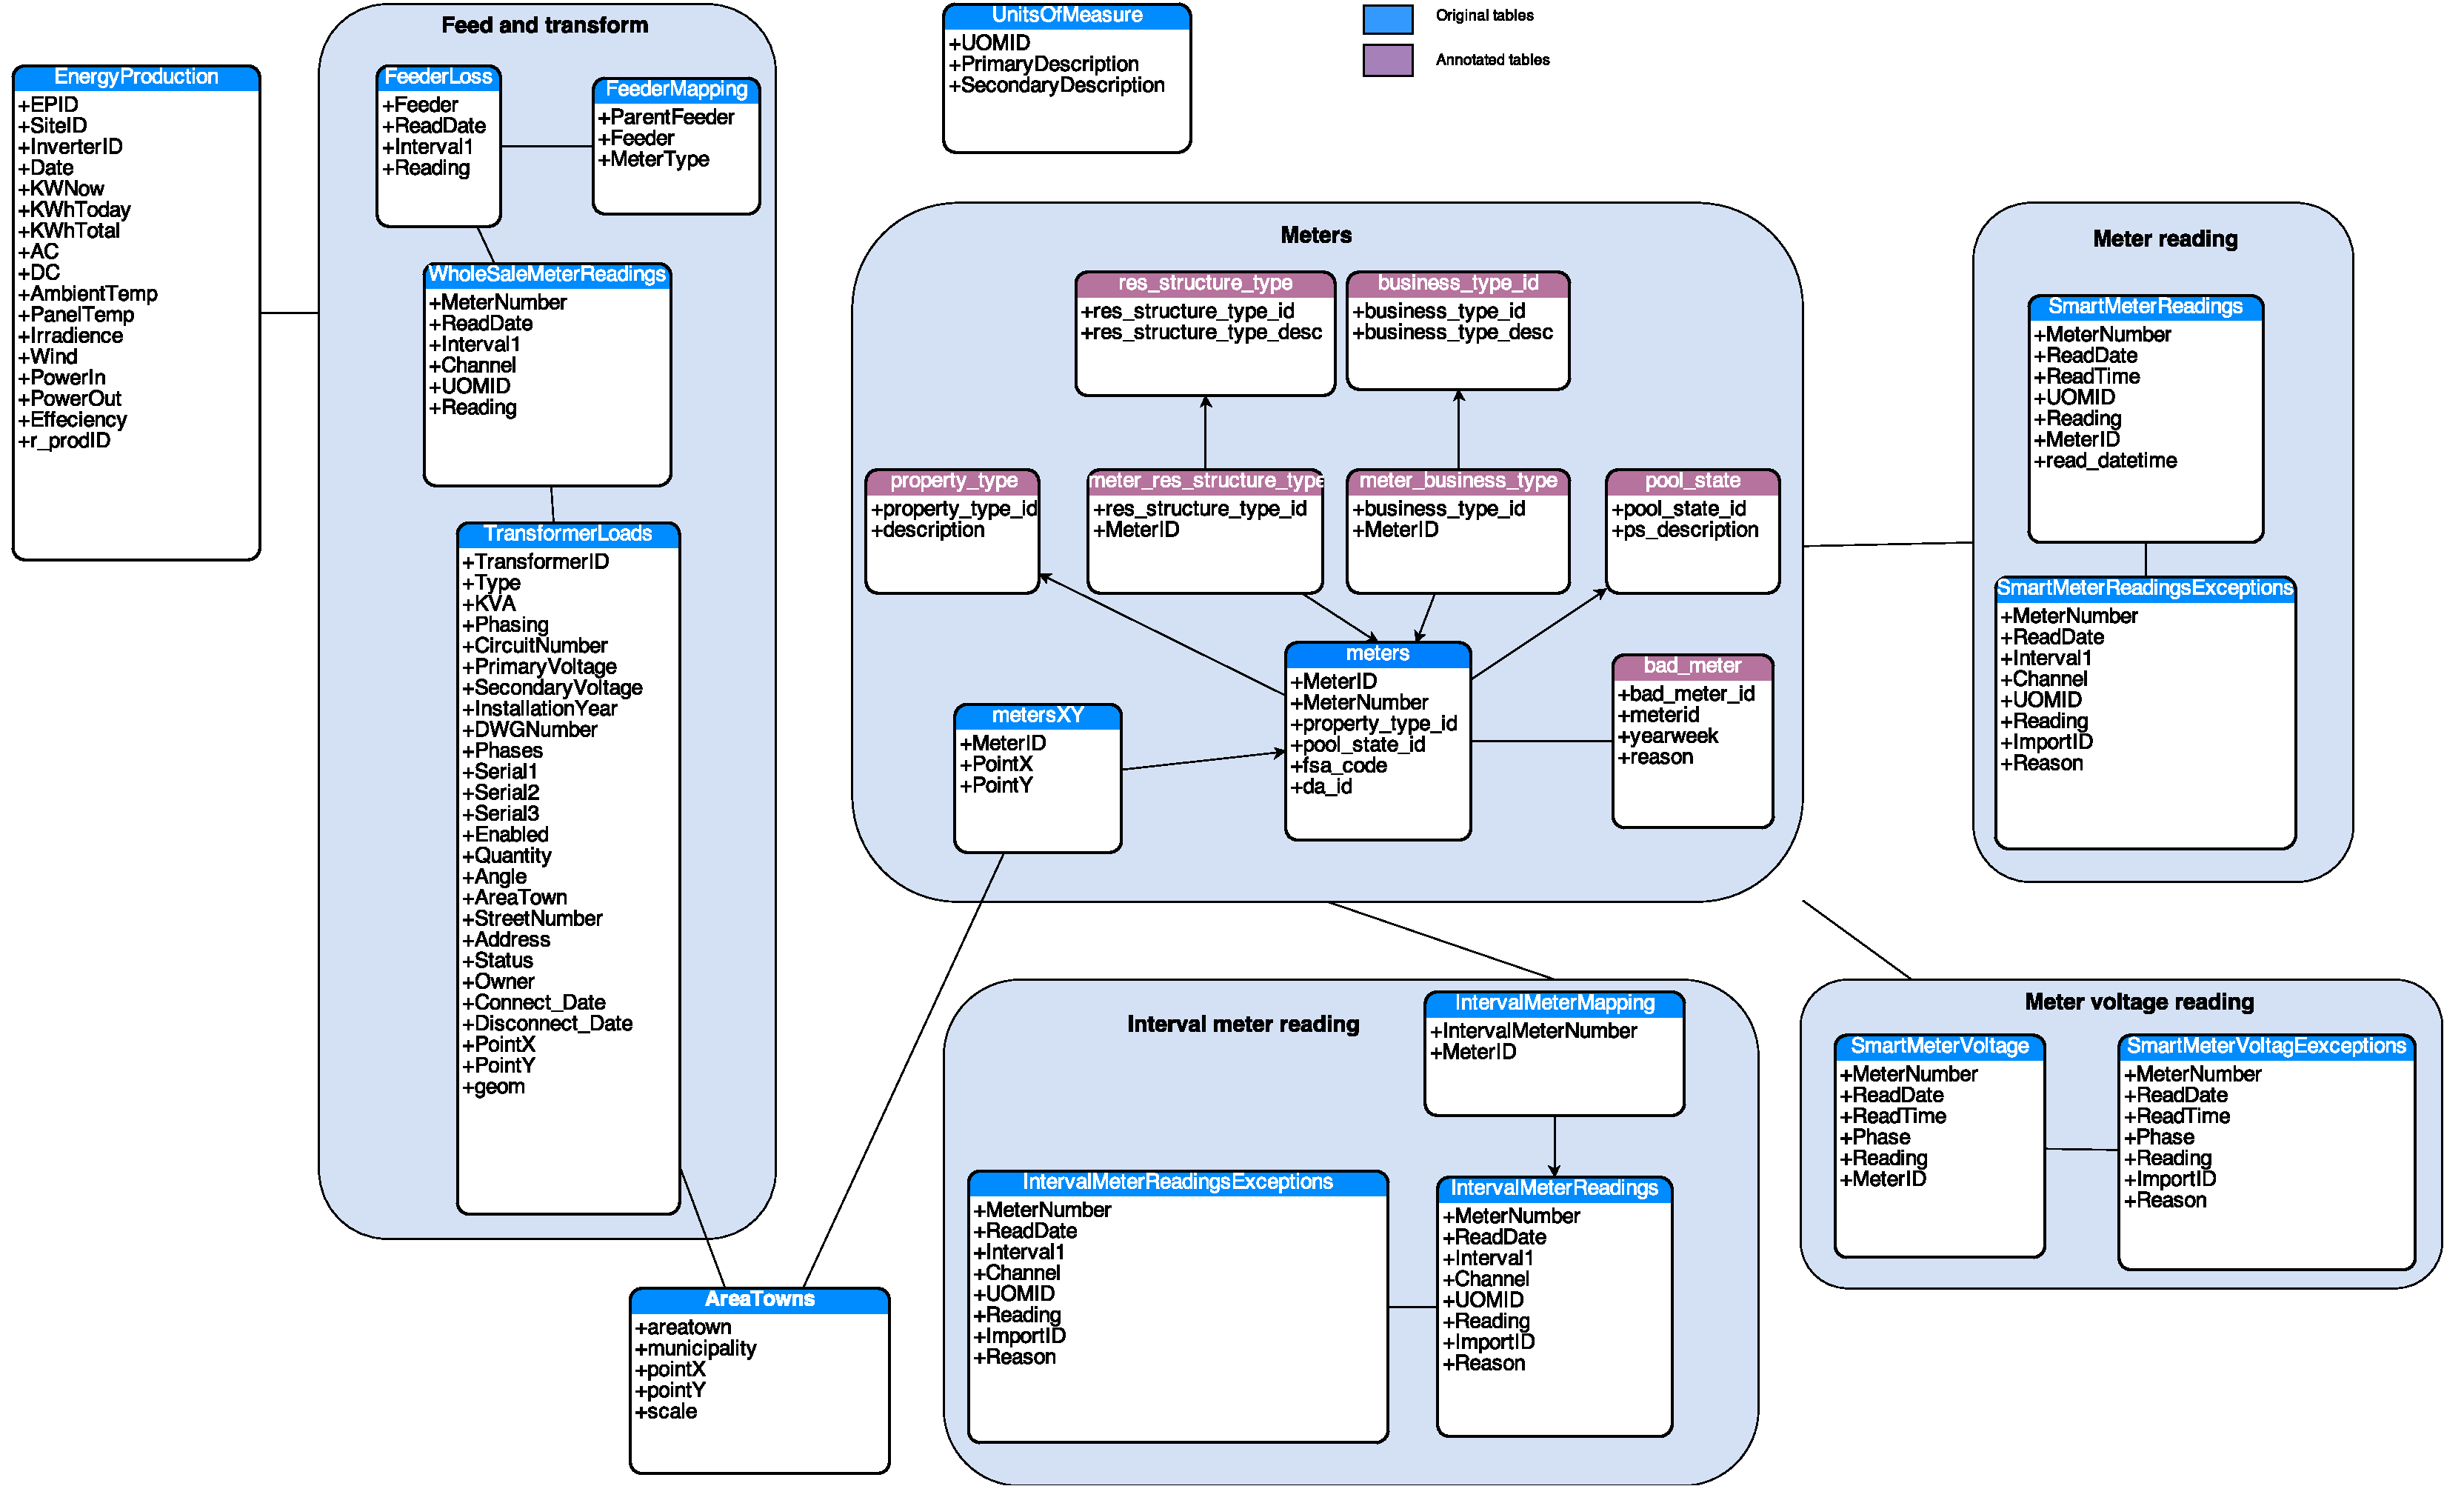
\includegraphics[width=1.1\textwidth]{images/essex_annotated}
\caption{Annotated ESSEX data}
\label{fig:essex_annotated}
\end{figure}

\subsection{Energy Production}
The data in this table is the metering data from the solar power systems at different sites. A solar power system exploits photovoltaic (PV) technology that converts sunlight into electrical energy.  \cite{solarsys} explains the mechanism. That is, PV technology uses solar cells made of semiconductor materials, such as silicon or germanium dosed with small amounts of impurities (typically metals or metalliods). When sunlight strikes a cell, a certain portion of its energy is absorbed with the semiconductor material, the absorbed energy knocks the electrons, and the loosen electrons flow freely under the influence of electric fields. Solar cells have inbuilt electric fields that force the freed electrons to flow in a certain direction. Metal contacts on the top and bottom of the PV cell enable the cell to generate a current in an external circuit. This current, together with the cell's voltage (which is a result of its in-built electric fields), defines the power (or wattage) that a solar cell can produce. This {\em direct current (DC)} can be used to recharge batteries, and run direct current devices, or can be converted via {\em inverters} into {\em alternating current (AC)}, the form of electricity most commonly used in homes, offices and industry.  




\begin{table}[htp]
\centering
\caption{EnergyProduction}
\begin{tabular}{|l|c|l|p{8.5cm}|}
 \hline
 {\bf Field}       & {\bf Type} & {\bf Example}     & {\bf Description } \\ \hline
 EPID        & int(11)   &1 & Sorrogate key of energy production \\ \hline
 SiteID      & int(11)   &1 &  The site of solar power system\\  \hline
 InverterID  & int(11)   &1 &  The inverter for converting the direct current to alternate current\\ \hline
 Date        & timestamp &2010-04-26 15:35:49 & The timestamp of metering the data. Here it reads every 5 minutes \\ \hline
 KWNow       & float     & 2.593& The reading at a point of the time  \\ \hline
 KWhToday    & float     & 20& The accumulated reading of a site of today \\  \hline
 KWhTotal    & float     &2491 & The accumulated reading of a site  \\ \hline
 AC          & float     & 256&  The alternative current after convertion \\ \hline
 DC          & float     &325 & The produced direct current of  electrons\\ \hline
 AmbientTemp & float     &18 &  The ambient air temperature around solar panel. The efficiency of PV can be affected by its operating temperature, which is primarily a product of the ambient air temperature as well as the level of sunlight. High ambient temperature could lower the energy generation efficiency.  \\ \hline
 PanelTemp   & float     &35 & The temperature of panel. The efficiency could also be affected by the panel temperature \\ \hline
 Irradience  & float     &481 & Measure the spectral irradiance in units of watts per meter squared \\ \hline
 Wind        & float     &12 & The wind speed on the site of measure. The wind speed could be corelated to the efficiency  \\ \hline
 PowerIn     & float     &2915.25 & The power received from network\\ \hline
 PowerOut    & float     &2554.88 & The power exported to network \\ \hline
 Effeciency  & float     &87.64 & \\ \hline
 r\_prodID   & int(11)   &1999693 & Energy production ID\\ \hline
\end{tabular}
\end{table}
The table \texttt{EnergyProduction} contains 50 sites' data, and the data granularity is 5 minutes, 2,929,404 records in total.  The measures of this table include the generated energy, \ie, \texttt{KWNow, KWhToday, KWhTotal}, the ambient and panel temperatures, irradience, efficiency, and wind. The dimensions include the sites of the solar power systems, the time, and the inverter of converting DC to AC. From this table we could ask some business questions from different perspectives (dimensions), and do the forecasting and correlation analysis. For example, to view the energy production for each of the inverters in time series fashion, study the impact of wind speed, panel and ambient, irradiance to the energy generation efficiency (by correlation), and  do the forecasting, etc.

\subsection{Feed and transform}
The power can be traded in the energy market. A utility company can buy the power from the market, and sell to the customers of a region, which is called {\em wholesale}.  The power is distributed through electricity distribution network from transmission systems  to the customers. Typically, the distribution network includes medium-voltage power lines, substations and transformers, low-voltage distribution wiring and meters (see Fig.~\ref{fig:distnetwork} from \cite{distnetwork}).  A distribution substation receives power from one or more transmission or sub-transmission lines at the corresponding transmission or sub-transmission voltage level,  and provides the power to one or more distribution feeders that originate from the substation.  Most feeders emanate radially from the substation to supply the load.  Some feeding loss occurs when the power is transferred from a substation to another substation. Typically, urban and suburban distribution is done with three-phase systems to serve both residential, commercial, and industrial loads. Distribution in rural areas may be only single-phase if it is not economical to install three-phase power for relatively few and small customers \cite{Brown}.
\begin{figure}[htp]
\centering
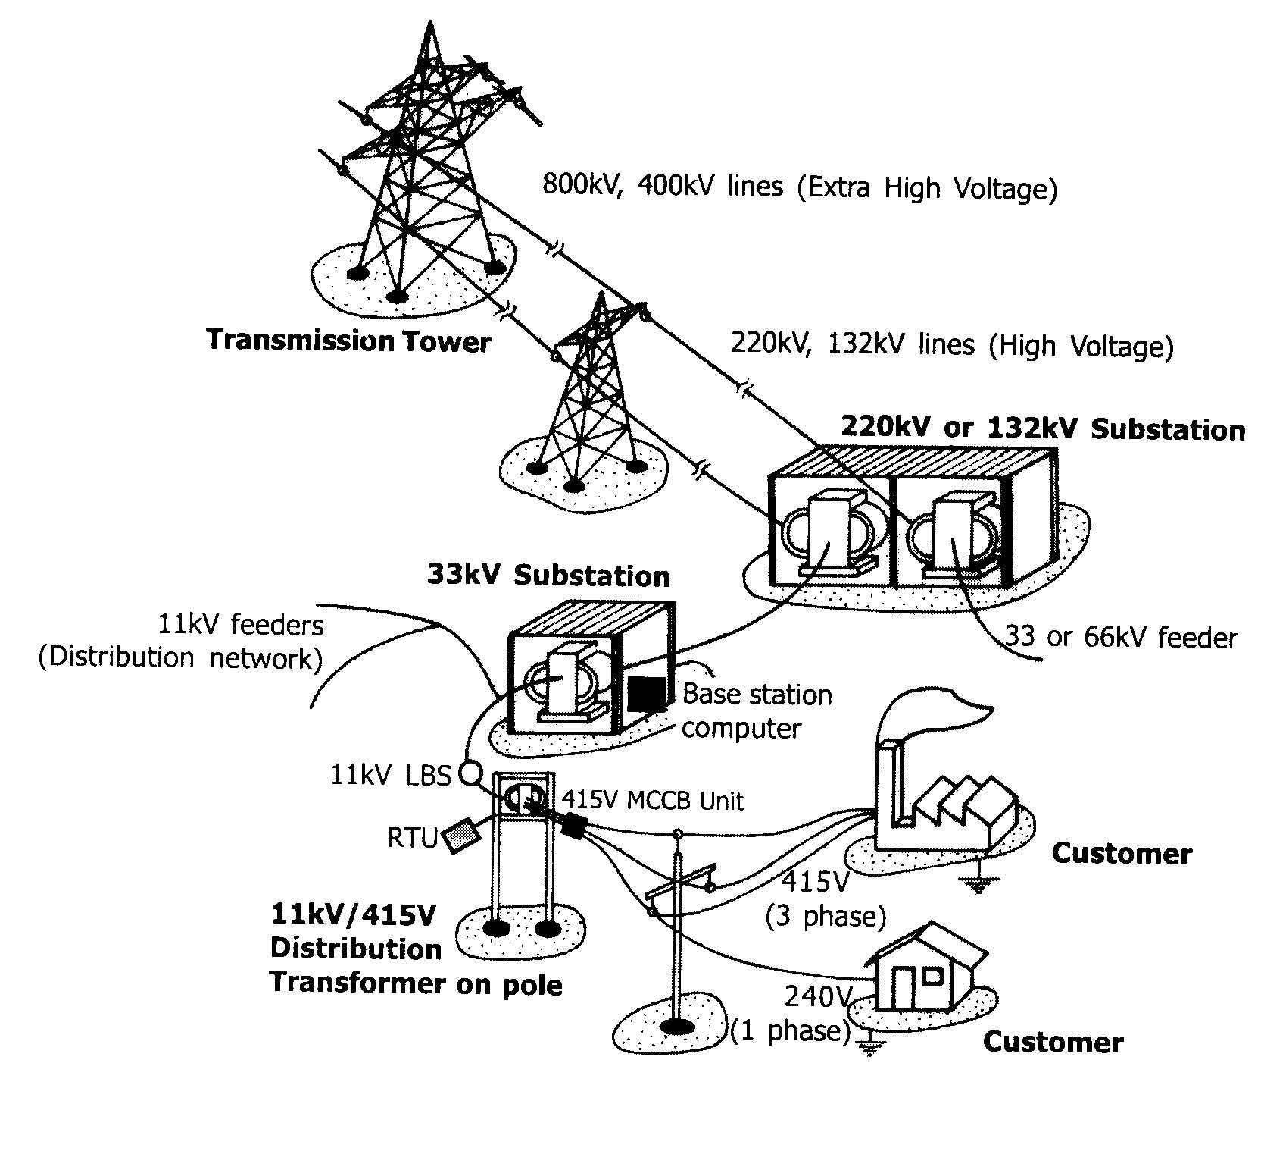
\includegraphics[width=0.7\textwidth]{images/distnetwork}
\caption{Electricity Distribution Network}
\label{fig:distnetwork}
\end{figure}

 The \texttt{WholesaleMeterReadings} table contains the wholesale data of utility companies. The metering data for each channel is read at one-hour interval per day, and each read was repeated for 30 times (a transformer has 4 isolation transformer units, Channels, which are read separately). The data in \texttt{FeederMapping}  describes the hierarchy structure of feeders, \ie, a substation and its children.  \texttt{FeederLoss} collects the  feeding loss read at one-hour interval per day.  \texttt{TransformerLoads}  describes the load of transformers, Circuit number, Phases, angle, address, and the geography locations etc. The transformation load is collected at one-hour interval per day. But, note that in this table there are 22 columns without any values (marked by ``N/A").


\begin{table}[htp]
\centering
\caption{WholesaleMeterReadings}
\begin{tabular}{|l|c|l|p{10cm}|}
 \hline
 {\bf Field}       & {\bf Type} & {\bf Example}     & {\bf Description } \\ \hline
MeterNumber&int(11)& 200700539 & Meter number  \\ \hline
ReadDate   &date   & 2011-09-01 & The reading date  \\ \hline
Interval1  &int(11)& 1 & The interval of reading meter, 4 channels in total  \\ \hline
Channel    &int(11)& 1 & Transformer channel  \\ \hline
UOMID      &int(11)& 1 &   \\ \hline
Reading    &int(11)& 1249 &  The value of the reading \\ \hline
\end{tabular}
\end{table}


\begin{table}[htp]
\centering
\caption{FeederMapping}
\begin{tabular}{|l|c|l|p{9.2cm}|}
 \hline
 {\bf Field}       & {\bf Type} & {\bf Example}     & {\bf Description } \\ \hline
ParentFeeder&varchar(250)&23M4  & Parent feeder ID  \\ \hline
Feeder      &varchar(250)&FSF1  & The feeder ID  \\ \hline
MeterType   &varchar(250)& SM &  Meter type \\  \hline
\end{tabular}
\end{table}



\begin{table}[htp]
\centering
\caption{FeederLoss}
\begin{tabular}{|l|c|l|p{8.5cm}|}
 \hline
 {\bf Field}       & {\bf Type} & {\bf Example}     & {\bf Description } \\ \hline
Feeder   &varchar(250)& 23M3 & Feeder ID  \\ \hline
ReadDate &timestamp   & 2012-06-01 00:00:00 &  The date of read \\ \hline
Interval1&int(11)     & 1 &  The interval of reading. It is 1-hour interval from 0 to 23 \\ \hline
Reading  &float       &-0.898  & The value of reading  \\ \hline
\end{tabular}
\end{table}


\begin{table}[htp]
\centering
\caption{TransformerLoads}
\begin{tabular}{|l|c|l|p{8.5cm}|}
 \hline
 {\bf Field}       & {\bf Type} & {\bf Example}     & {\bf Description } \\ \hline
TransformerID    &int(11)      & 9327 &  The transformer ID \\ \hline
Type             &date         & 2011-04-03 &  The date of read  \\ \hline
KVA              &float        & 0 & The interval of read, 0--23  \\ \hline
Phasing          &float        & 2.05 & The phase value of electricity  \\ \hline
CircuitNumber    &varchar(250) & N/A &   \\ \hline
PrimaryVoltage   &varchar(250) & N/A &   \\ \hline
SecondaryVoltage &varchar(250) & N/A &   \\ \hline
InstallationYear &varchar(250) & N/A &   \\ \hline
DWGNumber        &varchar(250) & N/A &   \\ \hline
Phases           &varchar(250) & N/A &   \\ \hline
Serial1          &varchar(250) & N/A &   \\ \hline
Serial2          &varchar(250) & N/A &   \\ \hline
Serial3          &varchar(250) & N/A &   \\ \hline
Enabled          &varchar(250) & N/A &   \\ \hline
Quantity         &varchar(250) & N/A &   \\ \hline
Angle            &varchar(250) & N/A &   \\ \hline
AreaTown         &varchar(250) & N/A &   \\ \hline
StreetNumber     &varchar(250) & N/A &   \\ \hline
Address          &varchar(250) & N/A &   \\ \hline
Status           &varchar(250) & N/A &   \\ \hline
Owner            &varchar(250) & N/A &   \\ \hline
Connect\_Date     &date         & N/A &   \\ \hline
Disconnect\_Date  &date         & N/A &   \\ \hline
PointX           &float        &N/A  &   \\ \hline
PointY           &float        & N/A &   \\ \hline
geom             &varchar(250) & N/A &   \\ \hline
\end{tabular}
\end{table}

\newpage

\subsection{Smart Meter Voltage Reading}
Transformers transform medium-high voltage power to low voltage  before feeding to the customers. The levels of voltage around the world is different. For example, in North America the voltage value is between 100 and 127 volts, while in European countries it is between 220 and 240 volts. The voltage readings beyond this range are regarded as the exception.   \texttt{SmartMeterVoltage} contains the voltage readings of three phases collected at 15-minute interval per day, and the exceptional readings are added to \texttt{SmartMeterVoltageException} for each read. This table also contains the no. of exceptions. The fact is the readings, and the dimensions are the dates, time, phases, and meters.

\begin{table}[htp]
\centering
\caption{SmartMeterVoltage}
\begin{tabular}{|l|c|l|p{9cm}|}
 \hline
 {\bf Field}       & {\bf Type} & {\bf Example}     & {\bf Description } \\ \hline
MeterNumber&varchar(250)& EP00001280& Meter number  \\ \hline
ReadDate   &date        &2011-12-21 &   \\ \hline
ReadTime   &time        &00:00:15 & The reading time interval in each day, 15-minute interval  \\ \hline
Phase      &int(11)     &2 & The power phases:  0, 1 and 2  \\ \hline
Reading    &float       &240.837 & The value of voltage  \\ \hline
MeterID    &int(11)     &19931 &   \\ \hline
\end{tabular}
\end{table}

\begin{table}[htp]
\centering
\caption{SmartMeterVoltageException}
\begin{tabular}{|l|c|l|p{9cm}|}
 \hline
 {\bf Field}       & {\bf Type} & {\bf Example}     & {\bf Description } \\ \hline
MeterNumber&varchar(250)& EP00018137&  Meter number \\ \hline
ReadDate   &date        &2011-12-21 & Reading date  \\ \hline
ReadTime   &time        &00:00:00 & The reading time  \\ \hline
Phase      &float       &0 & The power phases:  0, 1 and 2   \\ \hline
Reading    &float       &608.075 & The value of voltage  \\ \hline
ImportID   &int(11)     &2346 &   \\ \hline
Reason     &int(11)     &2 &   \\ \hline
\end{tabular}
\end{table}

\newpage
\subsection{Smart Meter Reading}
The tables in this category hold the power data consumed by customers.  \texttt{Meters} contains the mappings of  \texttt{MeterID} to \texttt{MeterNumber}.  \texttt{SmartMeterReadings} is holding the meter reading of {\em 1-minute} interval of each  meter, and the exception readings are hold in \texttt{SmartMeterReadingsExceptions}. The geography information of meters is  in  \texttt{MeterXY}, including the longitude and latitude on map. The fact is the meter readings, and the dimensions are date, time, and  meter ID, and location.
\begin{table}[htp]
\centering
\caption{Meters}
\begin{tabular}{|l|c|l|p{10cm}|}
 \hline
 {\bf Field}       & {\bf Type} & {\bf Example}     & {\bf Description } \\ \hline
MeterID    &int(11)& 19419&  Meter ID \\ \hline
MeterNumber&int(11)& 1&  Meter number \\ \hline
\end{tabular}
\end{table}
\begin{table}[htp]
\centering
\caption{SmartMeterReadings}
\begin{tabular}{|l|c|l|p{9cm}|}
 \hline
 {\bf Field}       & {\bf Type} & {\bf Example}     & {\bf Description } \\ \hline
MeterNumber&varchar(250)&EP00010116 & Meter number  \\ \hline
ReadDate   &date        &2010-10-29&  Reading date \\ \hline
ReadTime   &time        &00:04:00 &  Read time, at 1-minute interval \\ \hline
UOMID      &int(11)     &1 &   \\ \hline
Reading    &float       &0.74 &  The value of reading \\ \hline
MeterID    &int(11)     &22220 &  Meter ID \\ \hline
\end{tabular}
\end{table}
\begin{table}[htp]
\centering
\caption{SmartMeterReadingsExceptions}
\begin{tabular}{|l|c|l|p{8.5cm}|}
 \hline
 {\bf Field}       & {\bf Type} & {\bf Example}     & {\bf Description } \\ \hline
MeterNumber&int(11)  &323 & Meter number  \\ \hline
ReadDate   &timestamp&2011-03-03 00:00:00 & Reading date  \\ \hline
Interval1  &int(11)  &500 &   \\ \hline
Channel    &int(11)  &1 &  A smart meter typically has several channels that user can program for different tariff rates \\ \hline
UOMID      &int(11)  &1 &   \\ \hline
Reading    &int(11)  &694 &  The value of exceptional reading \\ \hline
ImportID   &int(11)  &2 &  The import ID of the meter that has exceptional reading \\ \hline
Reason     &int(11)  &N/A & The number of reason  \\ \hline
\end{tabular}
\end{table}
\begin{table}[htp]
\centering
\caption{MetersXY}
\begin{tabular}{|l|c|l|p{11.2cm}|}
 \hline
 {\bf Field}       & {\bf Type} & {\bf Example}     & {\bf Description } \\ \hline
MeterID&int(11)&19420 &  Meter ID \\ \hline
PointX &int(11)&329888 & Longitude  \\ \hline
PointY &int(11)&4678339 &  Latitude \\ \hline
\end{tabular}
\end{table}

\newpage
\subsection{Interval Meter Reading}
Interval Meter Readings are  at 1-hour interval for each of the channels in a meter. Typically, a meter has multiple channels, each of which show a different tariff. A utility companies can set the rate of power in each channel. The readings are in \texttt{IntervalMeterReadings}. The exceptional readings are in \texttt{IntervalMeterReadings\-Exceptions}. Therefore, the fact is the meter readings that could be viewed from the dimensions, reading date, time, Channels, Meter ID and locations.

\begin{table}[htp]
\centering
\caption{IntervalMeterMapping}
\begin{tabular}{|l|c|l|p{9.2cm}|}
 \hline
 {\bf Field}       & {\bf Type} & {\bf Example}     & {\bf Description } \\ \hline
IntervalMeterNumber&int(11)&814110 & Interval meter number  \\ \hline
MeterID            &int(11)&19894 &  Meter ID \\ \hline
\end{tabular}
\end{table}
\begin{table}[htp]
\centering
\caption{IntervalMeterReadings}
\begin{tabular}{|l|c|l|p{8.7cm}|}
 \hline
 {\bf Field}       & {\bf Type} & {\bf Example}     & {\bf Description } \\ \hline
MeterNumber&int(11)  &816510 & Meter number  \\ \hline
ReadDate   &timestamp&2011-09-01 00:00:00 &  Reading date \\ \hline
Interval1  &int(11)  &1 & Read interval, 1hour  \\ \hline
Channel    &int(11)  &1 & A channel showing a tariff where the rate can be set  \\ \hline
UOMID      &int(11)  &1 &   \\ \hline
Reading    &int(11)  &306 & Reading   \\ \hline
ImportID   &int(11)  &29485 &   \\ \hline
Reason     &int(11)  &N/A &   \\ \hline
\end{tabular}
\end{table}
\begin{table}[htp]
\centering
\caption{IntervalMeterReadingsExceptions}
\begin{tabular}{|l|c|l|p{8.7cm}|}
 \hline
 {\bf Field}       & {\bf Type} & {\bf Example}     & {\bf Description } \\ \hline
MeterNumber&int(11)  &816510 &  Meter number \\ \hline
ReadDate   &timestamp&2011-09-01 00:00:00 & Reading date  \\ \hline
Interval1  &int(11)  &1 &   \\ \hline
Channel    &int(11)  &1 & A channel showing a tariff where the rate can be set  \\ \hline
UOMID      &int(11)  &1 &   \\ \hline
Reading    &int(11)  &306 & Reading  \\ \hline
ImportID   &int(11)  &29485 &   \\ \hline
Reason     &int(11)  &N/A &  Exceptional reason \\ \hline
\end{tabular}
\end{table}

\newpage
\subsection{Other Tables}
Both are self-explained.
\begin{table}[htp]
\centering
\caption{UnitsOfMeasure}
\begin{tabular}{|l|c|l|p{8.6cm}|}
 \hline
 {\bf Field}       & {\bf Type} & {\bf Example}     & {\bf Description } \\ \hline
UOMID               & int(11)     & 1 &   \\ \hline
PrimaryDescription  & varchar(250)&KWH  &   \\ \hline
SecondaryDescription& varchar(250)&KW  &   \\ \hline
\end{tabular}
\end{table}
%\vspace{-20pt}
\begin{table}[H]
\caption{AreaTowns}
\begin{tabular}{|l|c|l|p{10cm}|}
 \hline
 {\bf Field}       & {\bf Type} & {\bf Example}     & {\bf Description } \\ \hline
areatown    & varchar(250)& A1-TEC &   \\ \hline
municipality& varchar(250)& Tecumseh &   \\ \hline
pointx      & varchar(250)& N/A &   \\ \hline
pointy      & varchar(250)& N/A &   \\ \hline
scale       & varchar(250)& N/A &   \\ \hline
\end{tabular}
\end{table}



\newpage
\section{Paper Reading}
The purpose of the weekly paper reading keeps me update the algorithms of data analysis and forecasting in energy. Followings are the papers I read this week.

\begin{itemize}
\item {\bf L.~Wang, L. Tanm  C.~Yu, and Z.~Wu. ``Study and Application of Non-Linear Time Series Prediction in Ground Source Heat Pump System". In {\em Proc. of CECNet}, pp. 3522--3525, 2012.}

Lu \et uses the two different algorithms,(SMOreg) Sequential Minimal Optimization for Regression \cite{li} and M5P(model tree) \cite{yang}, to do the forecasting of geothermal energy utilization of ground source heat pump system, which is the non-linear prediction. They argued that the selected two algorithms have better accuracy  than the other algorithms used in linear prediction, such as Microsoft time series, AR model, Cloud Model, etc. But, the paper does not compared with any of these algorithms. Instead, they test the two selected algorithms using the real data sets, and find that M5P shows a better accuracy comparing with SMOreg.

\item {\bf S.~Murugesan, J.~Zhang, and V.~Vittal. ``Finite State Markov Chain Model for Wind Generation Forecast: A Data-driven Spatiotemporal Approach". In {\em Proc. of ISGT}, pp. 1--8, 2012.}

This paper uses Markov chain model to forecast the aggregate power output from a wind farm. The model considers both spatial and temporal dynamics of wind power output of turbines in the farm. The temporal dynamics of the aggregate wind power is analyzed using auto-regression, while taking into account the diurnal non-stationarity and the seasonality.

\item {\bf D.~Tsoumakos, and C.~Mantas. ``The Case for Multi-engine Data Analytics". \url{http://www.cslab.ece.ntua.gr/~dtsouma/index_files/MEMS_mhpc2013.pdf}}

This is the position paper that envisions an analytics platform with Multi-Engine Management System (MEMS). 
The authors first study the state-of-the-art technologies for data analytics today, and the challenges. They found that due to the diversity of the analytics requirements, the data sources, and the hardware conditions, etc.,  users typically use different systems to do their analytics. They think it is desirable to build a unified analytics system for managing, executing and monitoring multiple, complex jobs. But, inside the system there lies multiple Management Systems that provide adaptive, cost-based and customizable resource management for  diverse resources.
\end{itemize}

\medskip
\begin{thebibliography}{1}
\bibitem{solarsys} 
J.~Toothman and S.~Aldous. ``How Solar Cells Work". \url{http://science.howstuffworks.com/environmental/energy/solar-cell1.htm} as of Nov 25, 2013.

\bibitem{distnetwork} 
http://www.iitk.ac.in/infocell/Archive/dirimg/power.jpg as of  Nov 25, 2013.

\bibitem{Brown} 
R.~E.~Brown,  ``Electric Power Distribution Reliability". Marcel Dekker, Inc., 2002.

\bibitem{li}
 C.~Li, L.~Jiang. ``Using Locally weighted learning to
improve SMOreg for regression[R]". Hubei: PRICAI 2006,2006:375–384.

\bibitem{yang}
J.~Yang, Y.~Zhai, D.~Xu, et al. ``SMO Algorithm applied in
time series model building and forecast". In {\em Proc. of ICMLC}, 2007:2395-2400, 2012.

\end{thebibliography}



\end{document}
